%Overview of existing technology (hardware)

\chapter{Overview of Existing Technology}
\section{PLC Hardware Controller Implementations}
%link to automotive statement: http://www.amci.com/tutorials/tutorials-what-is-programmable-logic-controller.asp
Programmable Logic Controllers (PLC) have been around for over 30 years and as a result there have been many iterations and designs. The original Programmable Logic Controllers were a quick way for automotive manufacturers to replace traditional relays with digital control. These relays were hooked up to power rails and inputs, and allowed for basic mechanical logic \cite{ebookmorris}. Due to their mechanical nature relays wore out over time causing the logic they were performing to fail. In addition, because hundreds to thousands could be used in a cabinet, it was also difficult to isolate the worn out part. Relays also proved to be inflexible when a small change was required to be added to the program, the entire plant was required to be taken offline in order to make the change. Halting large production plants is often extremely costly and thus eventually the relays were migrated out in favour of microcontrollers that can be reprogrammed on the fly. To this day modern PLC's still use graphical analogies of circuits and relays in order to construct their programmable logic. This visual language is now referred to as ladder logic due to the the finished program having a similar visual structure to a ladder. 

\begin{figure}[htp]
    \centering
    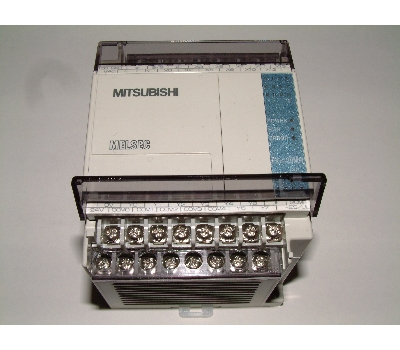
\includegraphics[width=\imgsmlphoto]{./images/c01_mitsubishiplc.jpg}
    \caption{Mitsubishi PLC All In One Unit \cite{img_c01_MitsubishiPlc}}
    \label{img:mitsubishiplc}
\end{figure}
Mitsubishi Automation (\ref{img:mitsubishiplc}), Siemens, and Omron are a few of the big producers of industry standard PLC's although the shape and form factor differ between manufacturers PLC's always consist of 3 distinct parts.  The input module, the main controller unit and the output module (please refer to Figure \ref{img:plcrender_1}). This separation exists due to varying requirements for analog inputs and different output capacity requirements in order to drive heavy machinery. I/O modules may consist of thermal-sensors, ambient light sensors, resistive sensors, or a direct connection to the external circuitry. The output module may also be composed of both analog and digital output pins.
\begin{figure}[htp]
    \centering
    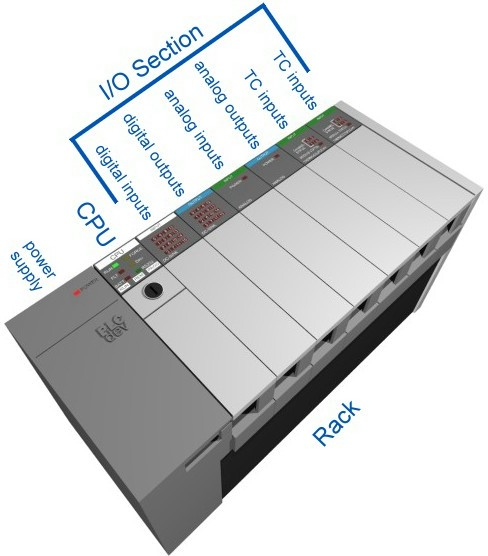
\includegraphics[width=\imgsmlphoto]{./images/c02_plcdev.jpg}
    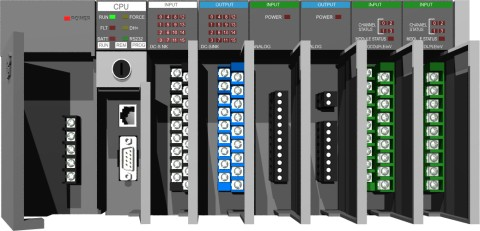
\includegraphics[width=\imgsmlphoto]{./images/c04_plcdev.jpg}
    \caption{3D Diagram of A Modular PLC \cite{img_c02_PlcDev,img_c04_PlcDev}}
    \label{img:plcrender_1}
\end{figure}

\pagebreak
%source http://www.sea.siemens.com/step/templates/lesson.mason?plcs:2:3:1
Programs that are executed from the main PLC control unit do so in iterations. An iteration of execution is referred to as a scan. Each scan is further broken up into 4 phases: Self-Test, Input scan, Logic solve / scan, and Output scan. Figure \ref{fig:plcexecution} shows the order in which each of these steps are executed. The jobs performed in each step is described in more detail below:
\begin{figure}[htb]
    \centering
    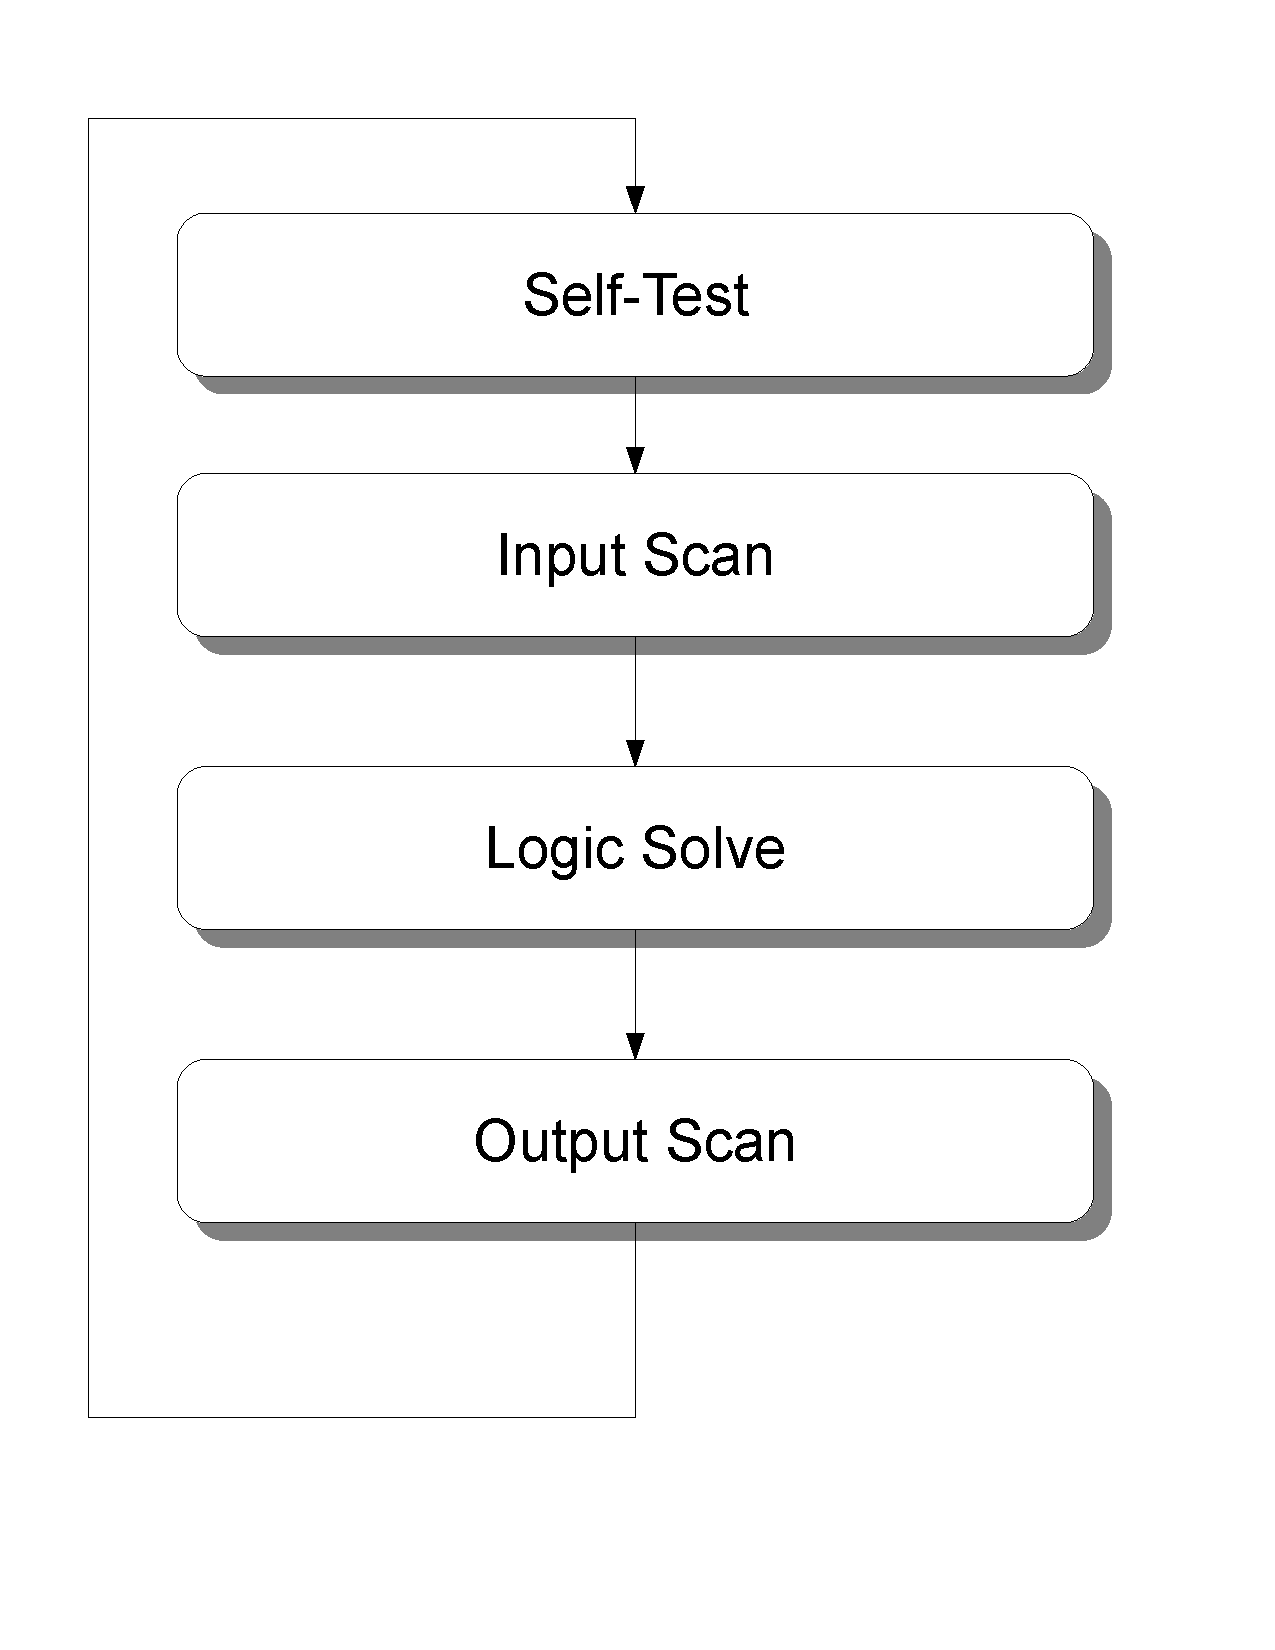
\includegraphics[width=\imgmedphoto]{./images/plcexecution.pdf}
    \caption{PLC Execution Loop}
    \label{fig:plcexecution}
\end{figure}

\begin{itemize}
	\item\textbf{Self-Test:} All PLC's contain self diagnostic routines, this includes communication checks between the main control unit and the I/O modules. If a fault is found it is handled here before any of the execution is allowed to proceed.
	\item\textbf{Input Scan:} All inputs both from the input modules and from the internal memory are read. This is done in a single step to make sure that all future calculations for the currently executing scan has consistent data. You may note that updates are not read during logic solve and will be delayed until the next input scan.
	\item\textbf{Logic Solve / Scan:} Calculations and computations from the user programs are computed in this step. If values are to be stored back into internal registers they are now put into temporary registers. Similarly if external output is required it is written to a temporary internal register that will hold the output until the output phase is executed.
	\item\textbf{Output Scan:} Internal temporary registers are written to their destination registers in one step. External outputs take on the values held by their associated temporary registers. All outputs also take place in one step and the outcome is that it appears that all outputs change simultaneously.
\end{itemize}

Each of these phases are modelled as if executions within them happen concurrently thus, the order of individual instructions in each phase is not important. All of this is done since Ladder Logic (please see section \ref{section:ladderlogic}) executes concurrently on multiple rungs since it is based off of electrical circuitry. Internally however PLC's are sequential machines with an deterministic order in which instructions are executed. This is a side effect of using microcontrollers in the main control unit instead of relays and circuitry. Many temporary registers are used to store inputs and outputs so that at the beginning each phase they can be latched in one step. This makes the reading of multiple inputs and outputs occur concurrently.

\begin{figure}[h]
    \centering
    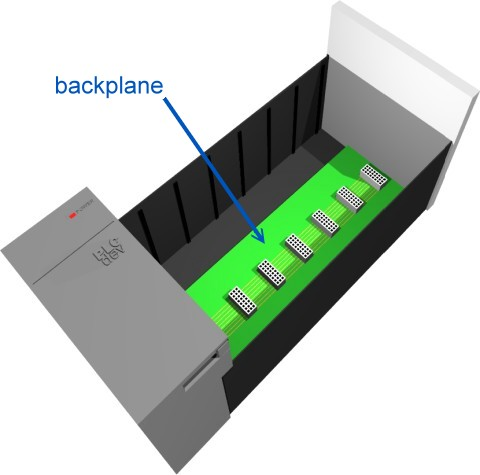
\includegraphics[width=\imgmedphoto]{./images/c03_plcdev.jpg}
    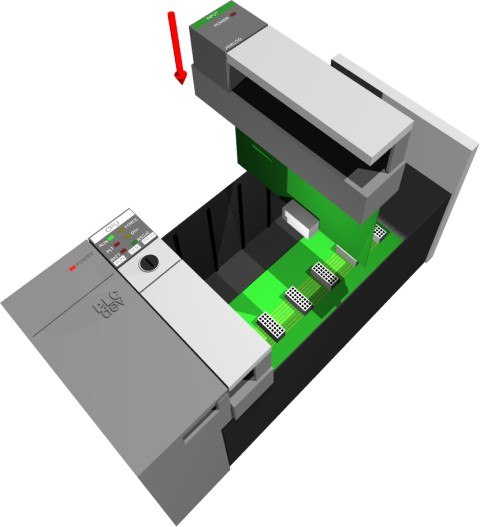
\includegraphics[width=\imgmedphoto]{./images/c05_plcdev.jpg}
    \caption{3D Diagram of A Modular PLC With One Module Being Inserted \cite{img_c03_PlcDev,img_c05_PlcDev}}
    \label{img:plcrender_2}
\end{figure}

The input and output modules generally connect to the main module via serial links however some manufacturers also include network communication over standard shielded Ethernet\cite{rockwell_io,rockwell_tech_pub}. Generally serial communication is used more often when the input and output modules are at a close distance to the controller unit as in a modular PLC designs  (see Figure \ref{img:plcrender_2}). The network interface on the other hand is used when the input or output module needs to be located far away from the main controller unit \cite{rockwell_tech_pub} as is often the case in automated production facilities. Output modules are generally relay driven and the driving current is provided by a transistor connected to logic pins of the main controller. This is done to isolate the internal circuitry from the high current demands of driving heavy machinery \cite{plcapp}. Alternatively some circuits employ an opto-isolator circuitry to achieve the same effect. The trade off in this design is it will accommodate less current under load but has faster switching and overall better service life \cite{plcapp}. Analog outputs are obtained by passing a binary value through a digital to analog converter (DAC). A reference voltage is usually required in such configurations.

%source http://www.toolingu.com/class-450240-plc-inputs-and-outputs.html
All input and output modules contain some common  features which allow for modularity. Each I/O module is assigned a unique address so that the controller unit running the PLC program can access it. Each controller also has what is referred to as a backpane which contains the necessary connectors to connect to the bus so the CPU can access it. Most I/O modules have multiple channels where each channel is either a single ended wire or a differential pairs. Differential pairs can be commonly seen in analog input modules where it is preferable to compare a signal with the sensor's reference ground. This is done to avoid problems with the ground mismatch between the PLC's CPU and the sensor. Such a mismatch would produce an undesirable floating ground and would induce a permanent error on the input channel. Most modules are designed so that the external inputs and outputs are completely isolated from the CPU circuitry. As such, the CPU is connected to common ground via the serial bus while the input and output modules are usually connected to the power supply via a ground screw (usually marked ``common''). In analog input modules conversion circuitry must exist to convert the sensed input values into quantized values to be sent over the serial bus. The same is true for analog output modules but in reverse. In digital inputs conversion is not needed however circuitry still exists for isolation of the internal bus from the external input, and where applicable the module itself may perform noise correction before the actual input enters the PLC itself. In addition to individual modules some PLC manufacturers opted to have the I/O modules embedded into the main CPU unit. These are generally more commonly found in the micro sized PLC's and are generally less expensive then their expandable counterparts. Although externally they are not expandable internally the configuration of the input modules are actually identical.

%source ISBN 0-13-025603-X
Due to the varying requirements of manufacturing over the years a wide variety of I/O modules now exist to fill in every need a short list of common I/O modules for the Allen-Bradley SLC500 series of PLC's is given below \cite{slc500}.
\begin{itemize}
	\item \textbf{Analog Input Module:} Reads in analog voltages converts them into digital values and sends the information to the control unit.
	\item \textbf{Analog Output Module:} Takes in digital values and produces an appropriate analog voltage level.
	\item \textbf{ASCII Input Module:} These modules take in character information usually via serial links (RS-232) and convert them into a form the PLC controllers can understand\cite{slc500}.
	\item \textbf{ASCII Output Module:} Takes PLC information converts it to an character representation and sends it out via RS-232.
	\item \textbf{Barrel-Temperature Module:} This module monitors four zones of an autotuned PID heating or cooling unit for temperature control. Molding machines and extruder employ these modules for controlling barrel temperature while injecting material \cite{slc500}.
	\item \textbf{BCD Input Module:} This module reads in inputs from devices that output binary-coded decimal (a method of representation where each decimal digit is represented by four bits). An example of such a device is a thumb wheel \cite{slc500}.
	\item \textbf{BCD Output Module:} Essentially does the reverse of the input module usually used for compatibility when devices expect data in BCD format.
	\item \textbf{Discrete Input Module:} These are isolated digital inputs.
	\item \textbf{Discrete Output Module:} These are isolated digital output modules.
	\item \textbf{Encoder Counter Module:} Keeps track of angular positioning of shafts.
	\item \textbf{Gray Encoder Module:} Receives grey-code signals from a device that produces grey-code.
	\item \textbf{High-Speed Counter-Encoder Module:} This type of module allows counting and encoding at a much faster rate than is normally possible inside a PLC program.
	\item \textbf{PID Module:} These modules enable the user to perform closed loop automatic control based on proportional integral and derivative values. If properly tuned the module can hold a process at the desired set point.
	\item \textbf{Synchronized Axes Module:} Provides logic to synchronize machines like hydraulic tailgate loaders, forging machines, and rolling-position operations.
	\item \textbf{Thermocouple Modules:} These modules allow the PLC to read temperatures of a process and will output usually with Celsius or Fahrenheit.
	\item \textbf{TTL Input Module:} Allows reading inputs from TTL devices such as most integrated circuits.
\end{itemize}

Programmable logic controllers can classified into three categories: Integrated such as a Mitsubishi Melsec FX-32MR seen in Figure \ref{img:mitsubishiplc}, Modular as seen in Figure \ref{img:plcrender_1}, and Large Scale automation. The integrated category includes small one board solutions generally better suited for low power or embedded applications. The modular category consists of PLC's that have a rack that houses the power supply, and several modular slots for both the microcontroller and various input and output modules.

Compact units such as the Melsec previously mentioned commonly have an input output port range from 8 - 24 these are not expandable due to its all-in-one nature. The Melsec unit has 2000 steps of execution memory. Each step can be loosely thought of as an instruction. However, the nature of ladder logic programming tends to obscure what a step is after it is compiled. The output capacity of these compact units can range anywhere from milliamps to a few amps. As an example the Melsec FX-32MR in Figure \ref{img:mitsubishiplc} can output a maximum of 8A on 4 of it's ports and only 2A on the remaining ports. Modular units on the other hand are able to scale to the diverse demands of operating heavy machinery by fitting them with high capacity output units.

